\documentclass[tikz,border=12pt]{standalone}
\usepackage{tikz}
\usetikzlibrary{positioning,arrows.meta,shapes.misc}
\usepackage{fontawesome5}
\begin{document}
	\begin{tikzpicture}[
		>={Stealth[length=6pt]},
		node distance=5.5cm and 5.5cm,
		state/.style={
			draw, rounded rectangle,
			minimum width=3.8cm, minimum height=1.4cm,
			align=center, font=\small\bfseries,
			line width=0.8pt, inner sep=6pt
		},
		normal/.style ={state, fill=blue!10,   draw=blue!50!black},
		eager/.style  ={state, fill=orange!20, draw=orange!70!black},
		forced/.style ={state, fill=green!12,  draw=green!50!black},
		lbl/.style={font=\footnotesize, align=center, text width=3.0cm},
		]
		
		%% States
		\node[normal] (N) {NORMAL MODE\\{\mdseries\itshape Skip Module ON}};
		\node[eager,  right=of N] (E) {EAGER MODE\\{\mdseries\itshape Skip Module suppressed, always RunDL}};
		\node[forced, below=2.8cm of N] (F) {FORCED CHECK\\{\mdseries\itshape RunDL once, reset skip\_streak}};
		
		%% N -> E  (fire via motion gate)
		\path[->, bend left=20, draw=red!70!black, line width=0.8pt]
		(N) edge node[above, lbl]{{\large \color{red}\faFire} detected \\ (Skip Module Enable, and Run DL)} (E);
		
		%% E -> N  (confirmed clear)
		\path[->, bend left=20, draw=teal!70!black, line width=0.8pt]
		(E) edge node[below, lbl]{non\_FireSmoke\_streak ${\geq}\,W_{\mathrm{clr}}$ (scene clear)} (N);
		
		%% N -> F  (skip streak)
		\path[->, bend right = 15, draw=gray!60!black, line width=0.8pt]
		(N) edge node[left, lbl, text width=2.6cm]{skip\_streak ${\geq}\,N_{\mathrm{chk}}$} (F);
		
		%% F -> N  (no fire)
		\path[->, bend right=15, draw=teal!70!black, line width=0.8pt]
		(F) edge node[right, lbl, text width=2.6cm]{{\large \color{red}\faFire} NOT detected (resume normal)} (N);
		
		%% F -> E  (fire during forced check)
		\path[->, draw=red!70!black, line width=0.8pt]
		(F) edge[out=0, in=270] node[right, lbl, xshift=0.2cm]{{\large \color{red}\faFire} detected (forced check)} (E);
		
		%% E -> E  self-loop
		\path[->, draw=orange!70!black, line width=0.8pt]
		(E) edge[out=60, in=120, looseness=5] node[above, lbl]{{\large \color{red}\faFire} detected (stay in eager)} (E);
		
	\end{tikzpicture}
\end{document}